\documentclass[12pt]{article}

\usepackage{geometry}
\usepackage{tikz}
\usetikzlibrary{mindmap}

\geometry{landscape, margin=1cm}

\begin{document}
\pagestyle{empty}
\begin{center}
    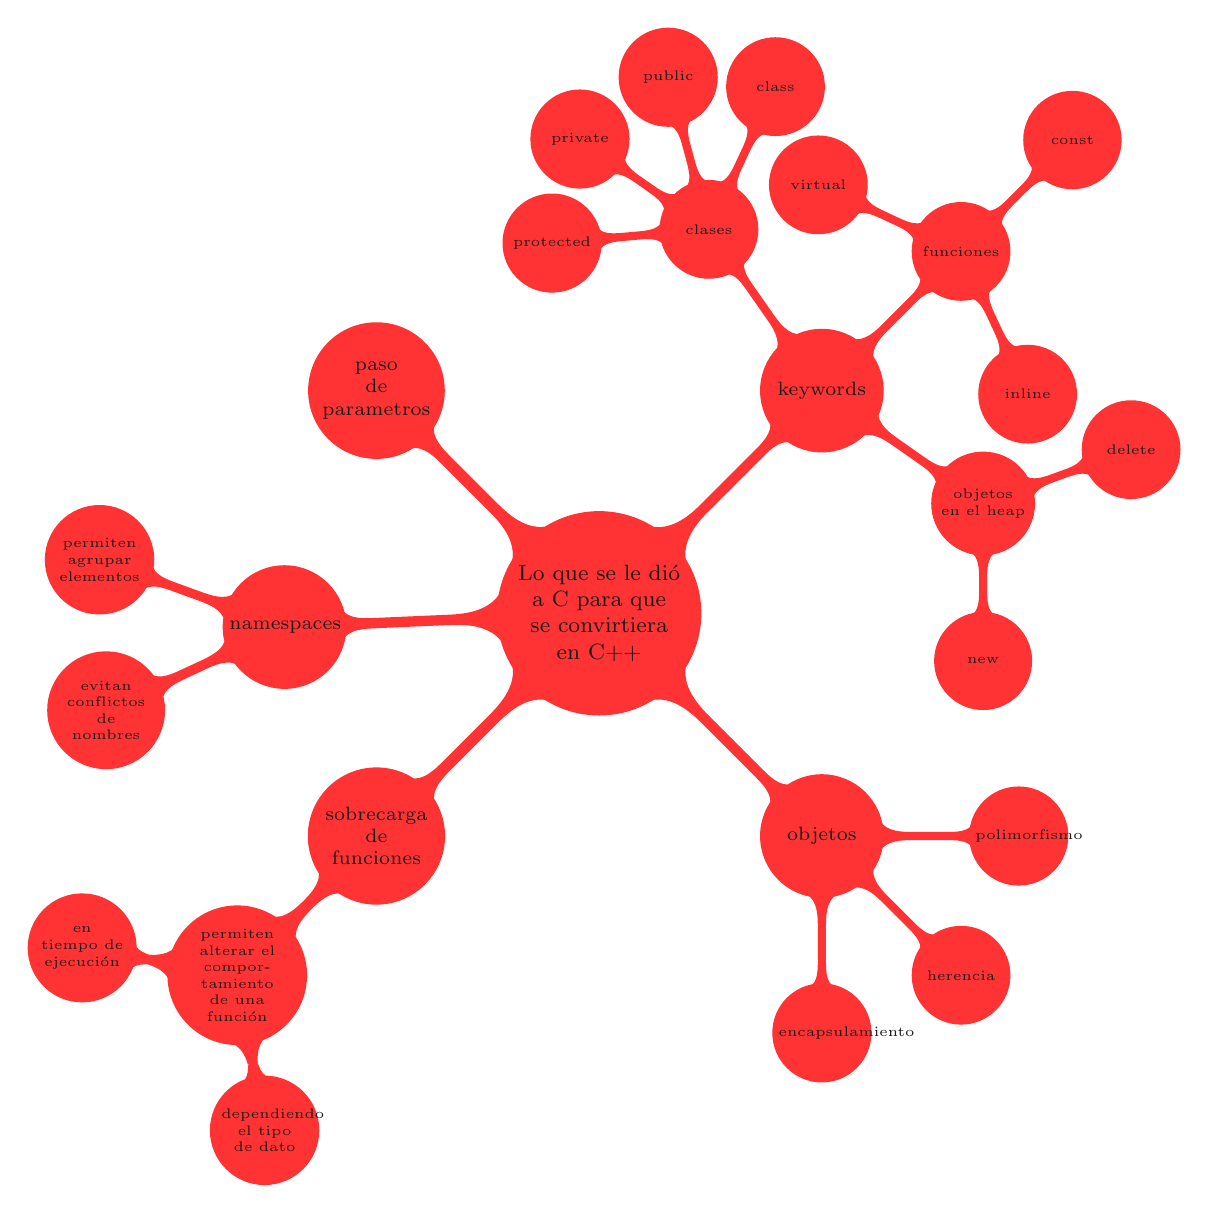
\begin{tikzpicture}[small mindmap, grow cyclic, every node/.style=concept, concept color=red!80, text=black!90,
        level 1/.append style={level distance=4cm, sibling angle=90},
        level 2/.append style={level distance=2.5cm, sibling angle=45},
        level 3/.append style={level distance=2cm, sibling angle=110}]
    \node{Lo que se le dió a C para que se convirtiera en C++}
        child { node { namespaces } }
        child { node { sobrecarga de\\ funciones }
            child { node { permiten alterar el comportamiento de una función }
                child { node { en tiempo de ejecución } }
                child { node { dependiendo el tipo de dato } }
            }
        }
        child { node { objetos }
            child { node { encapsulamiento } }
            child { node { herencia } }
            child { node { polimorfismo } }
        }
        child { node { keywords }
            child[sibling angle=80] { node { objetos en el heap }
                child { node { new } }
                child { node { delete } }
            }
            child[sibling angle=80] { node { funciones }
                child { node { inline } }
                child { node { const } }
                child { node { virtual } }
            }
            child[sibling angle=80] { node { clases }
                child[sibling angle=40] { node { class } }
                child[sibling angle=40] { node { public } }
                child[sibling angle=40] { node { private } }
                child[sibling angle=40] { node { protected } }
            }
        }
        child { node { paso\\ de\\ parametros } }
        child[sibling angle=217] { node { namespaces }
            child { node { permiten agrupar elementos } }
            child { node { evitan conflictos de nombres } }
        }
    ;
    \end{tikzpicture}
\end{center}
\end{document}
